\documentclass[10pt,a4paper]{article}

% ============================================================================
% PACKAGE IMPORTS
% ============================================================================
\usepackage[margin=12mm,top=13mm,bottom=13mm]{geometry}
\usepackage[utf8]{inputenc}
\usepackage[T1]{fontenc}
\usepackage{booktabs}
\usepackage{tabularx}
\usepackage{graphicx}
\graphicspath{{./}{../}{assets/}{../assets/}}
\usepackage{microtype}
\usepackage[hidelinks]{hyperref}
\usepackage{xcolor}
\usepackage{titlesec}
\usepackage{enumitem}
\usepackage{fancyhdr}
\usepackage{amsmath}
\usepackage{array}

% Table styling
\renewcommand{\arraystretch}{0.88}
\setlength{\tabcolsep}{3.5pt}

% Float spacing
\setlength{\floatsep}{3pt plus 1pt minus 1pt}
\setlength{\textfloatsep}{4pt plus 1pt minus 1pt}
\setlength{\intextsep}{3pt plus 1pt minus 1pt}

% ============================================================================
% IDENTITY PLACEHOLDERS (Zero Hardcoded PII)
% ============================================================================
\newcommand{\StudentID}{{{STUDENT\_ID}}}
\newcommand{\StudentNameEn}{{{STUDENT\_NAME\_EN}}}
\newcommand{\StudentNameVi}{{{STUDENT\_NAME\_VI}}}

% ============================================================================
% TYPOGRAPHY CONFIGURATION
% ============================================================================
\setlength{\parindent}{0pt}
\setlength{\parskip}{1.8pt}
\setlist{noitemsep, topsep=0.5pt, parsep=0pt, partopsep=0pt, leftmargin=*}

\titleformat{\section}{\large\bfseries}{\thesection}{0.8em}{}
\titleformat{\subsection}{\normalsize\bfseries}{\thesubsection}{0.8em}{}
\titleformat{\subsubsection}{\normalsize\itshape}{\thesubsubsection}{0.8em}{}

\titlespacing*{\section}{0pt}{3pt plus 1pt minus 1pt}{1.5pt plus 1pt minus 1pt}
\titlespacing*{\subsection}{0pt}{2.5pt plus 1pt minus 1pt}{1pt plus 1pt minus 1pt}
\titlespacing*{\subsubsection}{0pt}{2pt plus 1pt minus 1pt}{0.5pt plus 1pt minus 1pt}

% Header/Footer
\pagestyle{fancy}
\fancyhf{}
\fancyhead[L]{\small SE2026 Assignment 01 | Variant RE-027}
\fancyhead[R]{\small \StudentID}
\fancyfoot[C]{\thepage}
\renewcommand{\headrulewidth}{0.4pt}

% ============================================================================
% DOCUMENT METADATA
% ============================================================================
\title{\textbf{SE2026 Personal Assignment 1}\\
\large Topic AI-03: GitHub Project Coach for Student Teams\\
\large Variant RE-027: Personal-Data-Deletion-on-Request Policy}
\author{\StudentNameEn{} (\StudentNameVi)\\
Student ID: \StudentID\\
Team SE2026-T07}
\date{Submission Date: October 2026}

% ============================================================================
% BEGIN DOCUMENT
% ============================================================================
\begin{document}

\maketitle
\thispagestyle{fancy}

% Declaration of Accountability
\begin{center}
\fbox{\parbox{0.9\textwidth}{\centering\itshape
"I assume full responsibility for the content of this submission\\
and have declared my use of AI."
}}
\end{center}

\vspace{8pt}

% ============================================================================
% SECTION 1: EXECUTIVE CONTEXT
% ============================================================================
\section{Executive Context and Variant RE-027 Operational Constraints}

This submission analyzes the \textbf{Access Administrator} stakeholder perspective under the \textbf{Personal-Data-Deletion-on-Request} policy for the AI-03 GitHub Project Coach system. The variant is defined by three immutable operational parameters:

\begin{itemize}[leftmargin=*]
 \item \textbf{302 concurrent active users}: Peak-load concurrency ceiling for access-rights evaluations during policy re-evaluation cycles.
 \item \textbf{41-day audit retention limit}: Audit records must remain retrievable for forensic investigation for exactly 41 days, followed by mandatory automated purging.
 \item \textbf{20-hour change request response window}: Any data-deletion or access-revocation request must receive fulfillment confirmation within 20 elapsed hours (calendar clock, not business hours per ASSUMPTION-01).
\end{itemize}

The core operational dilemma is a three-way architectural tension: the Access Administrator must honor deletion requests, maintain a 41-day auditable trail satisfying security operations, and sustain operational stability for 302 concurrent users---all within a 20-hour response envelope. The deletion policy demands irreversible removal of personal identifiers, yet the audit retention mandate requires event attribution for 41 days. These obligations are mutually exclusive unless an architectural transformation (irreversible tokenization with stable surrogate keys) bridges the gap.

The submission adheres strictly to ISO/IEC/IEEE 29148 requirements terminology, maintains implementation independence (zero technology names in requirements), and records all AI-assisted artifacts with explicit human disposition auditing per ACM/IEEE engineering accountability standards.

% ============================================================================
% SECTION 2: SOFTWARE ENGINEERING IN THE AI ERA
% ============================================================================
\section{Software Engineering in the AI Era}

\subsection{Working Software vs. Reliable Software}

Generative AI systems produce code that compiles, passes unit tests, and deploys without immediate crash---yet fails under the operational constraints of Variant RE-027. Three failure vectors illustrate the divergence between \textit{working} and \textit{reliable} software:

\textbf{Race Conditions in Session Invalidation.} An AI-generated deletion pipeline may correctly remove a user's profile and emit a confirmation event, yet fail to atomically invalidate active sessions across 302 concurrent connections. Under peak load, the window between profile removal and session termination becomes a race: new access requests may be evaluated against stale tokens, granting access to a logically deleted identity. A unit test that mocks the session store in isolation cannot reproduce the timing interleavings of 302 concurrent sessions under a revocation storm.

\textbf{Incomplete Deletion Pipelines with Residual Metadata.} The deletion policy demands irreversible removal of personal identifiers. An AI-generated implementation may correctly tokenize the primary identity table while leaving foreign-key references, cached query results, or message-queue payloads intact. These residuals constitute direct PII exposure during the 41-day audit retention period. A test suite asserting "the user table is clean" will pass while the search index still returns the deleted user's email.

\textbf{SLA Deadline Drift Under Partial Degradation.} The 20-hour response window is absolute. An AI-generated escalation subsystem may correctly implement priority queues and notification templates, yet assume reliable network delivery. When the primary alert channel degrades, the system silently queues escalation tasks without triggering the fallback channel, causing requests to breach the SLA. A test asserting "an escalation event is created" will pass while the alert never reaches the Access Administrator.

In each case, the code executes without error. The failure is a violation of an operational guarantee that the test suite did not encode. Reliability requires that every operational constraint of the variant be expressed as a verifiable property and checked under realistic adversarial conditions.

\subsection{Locus of Engineering Responsibility}

The ACM Code of Ethics (Section 1.2) and IEEE Code of Ethics hold that engineers must "accept responsibility for their decisions and actions." Generative AI alters the mechanics of production but not the locus of accountability. When an AI generates a deletion pipeline that leaks PII into an audit log, the legal consequence falls on the deploying organization and the engineer who signed off on the release. The AI agent has no legal personhood, no professional license, and no capacity to suffer sanctions.

Under GDPR Article 24, the controller must implement appropriate technical measures and demonstrate compliance. An AI-generated artifact without a documented, human-verified assurance chain does not satisfy this requirement. The engineer's professional duty is to construct that assurance chain: to specify the required behavior, verify the implementation, and record the evidence. The AI is a tool, subject to the same scrutiny as any compiler or static analyzer. Responsibility cannot be delegated to the tool.

\subsection{Systematic AI Failure Modes and Countermeasures}

\begin{table}[htbp]
\centering
\scriptsize
\begin{tabularx}{\textwidth}{|l|X|X|}
\hline
\textbf{AI Failure Mode} & \textbf{RE-027 System Failure Manifestation} & \textbf{Deterministic Engineering Countermeasure} \\
\hline
\textbf{Semantic Hallucination} & AI generates phantom calls to non-existent API endpoints (e.g., \texttt{DELETE /api/compliance/purge}) and cites fictitious ISO clauses, introducing unhandled runtime dependencies. & Implementation-independent formal specification (ISO 29148); strict SAST dependency checking; static type validation. \\
\hline
\textbf{Edge-Case Blindness} & AI optimizes nominal paths, ignoring late requests at hour 19.5 with active session locks, causing deadlocks and silent SLA breaches beyond 20h. & Property-based testing simulating boundary clock arrivals (16h, 18h, 19.5h, 20h); automated multi-channel escalation alerts. \\
\hline
\textbf{Privacy Blindspots} & AI logs full request payloads (containing raw PII) into audit tables for debugging, violating the 41-day retention limit and privacy mandate. & Deterministic SAST linters prohibiting direct PII logging; irreversible pseudonymization before audit persistence; Day 42 purge. \\
\hline
\end{tabularx}
\caption{Systematic AI Failure Modes, Manifestations, and Engineering Countermeasures}
\label{tab:failure_modes}
\end{table}

\textbf{6-Layer Defense-in-Depth Pipeline:} (1) Formal Specification $\rightarrow$ (2) Property-Based Testing $\rightarrow$ (3) Static Analysis/SAST $\rightarrow$ (4) Human Audit Gates $\rightarrow$ (5) Bidirectional Traceability $\rightarrow$ (6) Full Load Testing (302 users). Failure in one layer is deterministically trapped by subsequent layers.

% ============================================================================
% SECTION 3: 1-WEEK AI-AUGMENTED SOFTWARE PROCESS
% ============================================================================
\section{1-Week AI-Augmented Software Process}

\subsection{Process Model Overview}

The process integrates AI-assisted drafting within a rigorously gated, human-accountable engineering discipline. Every AI artifact passes through explicit verification gates before advancement. The week is a single iteration from inception to release readiness, matching the 20-hour change-request window and the assignment's one-week workflow requirement.

\begin{figure}[htbp]
\centering
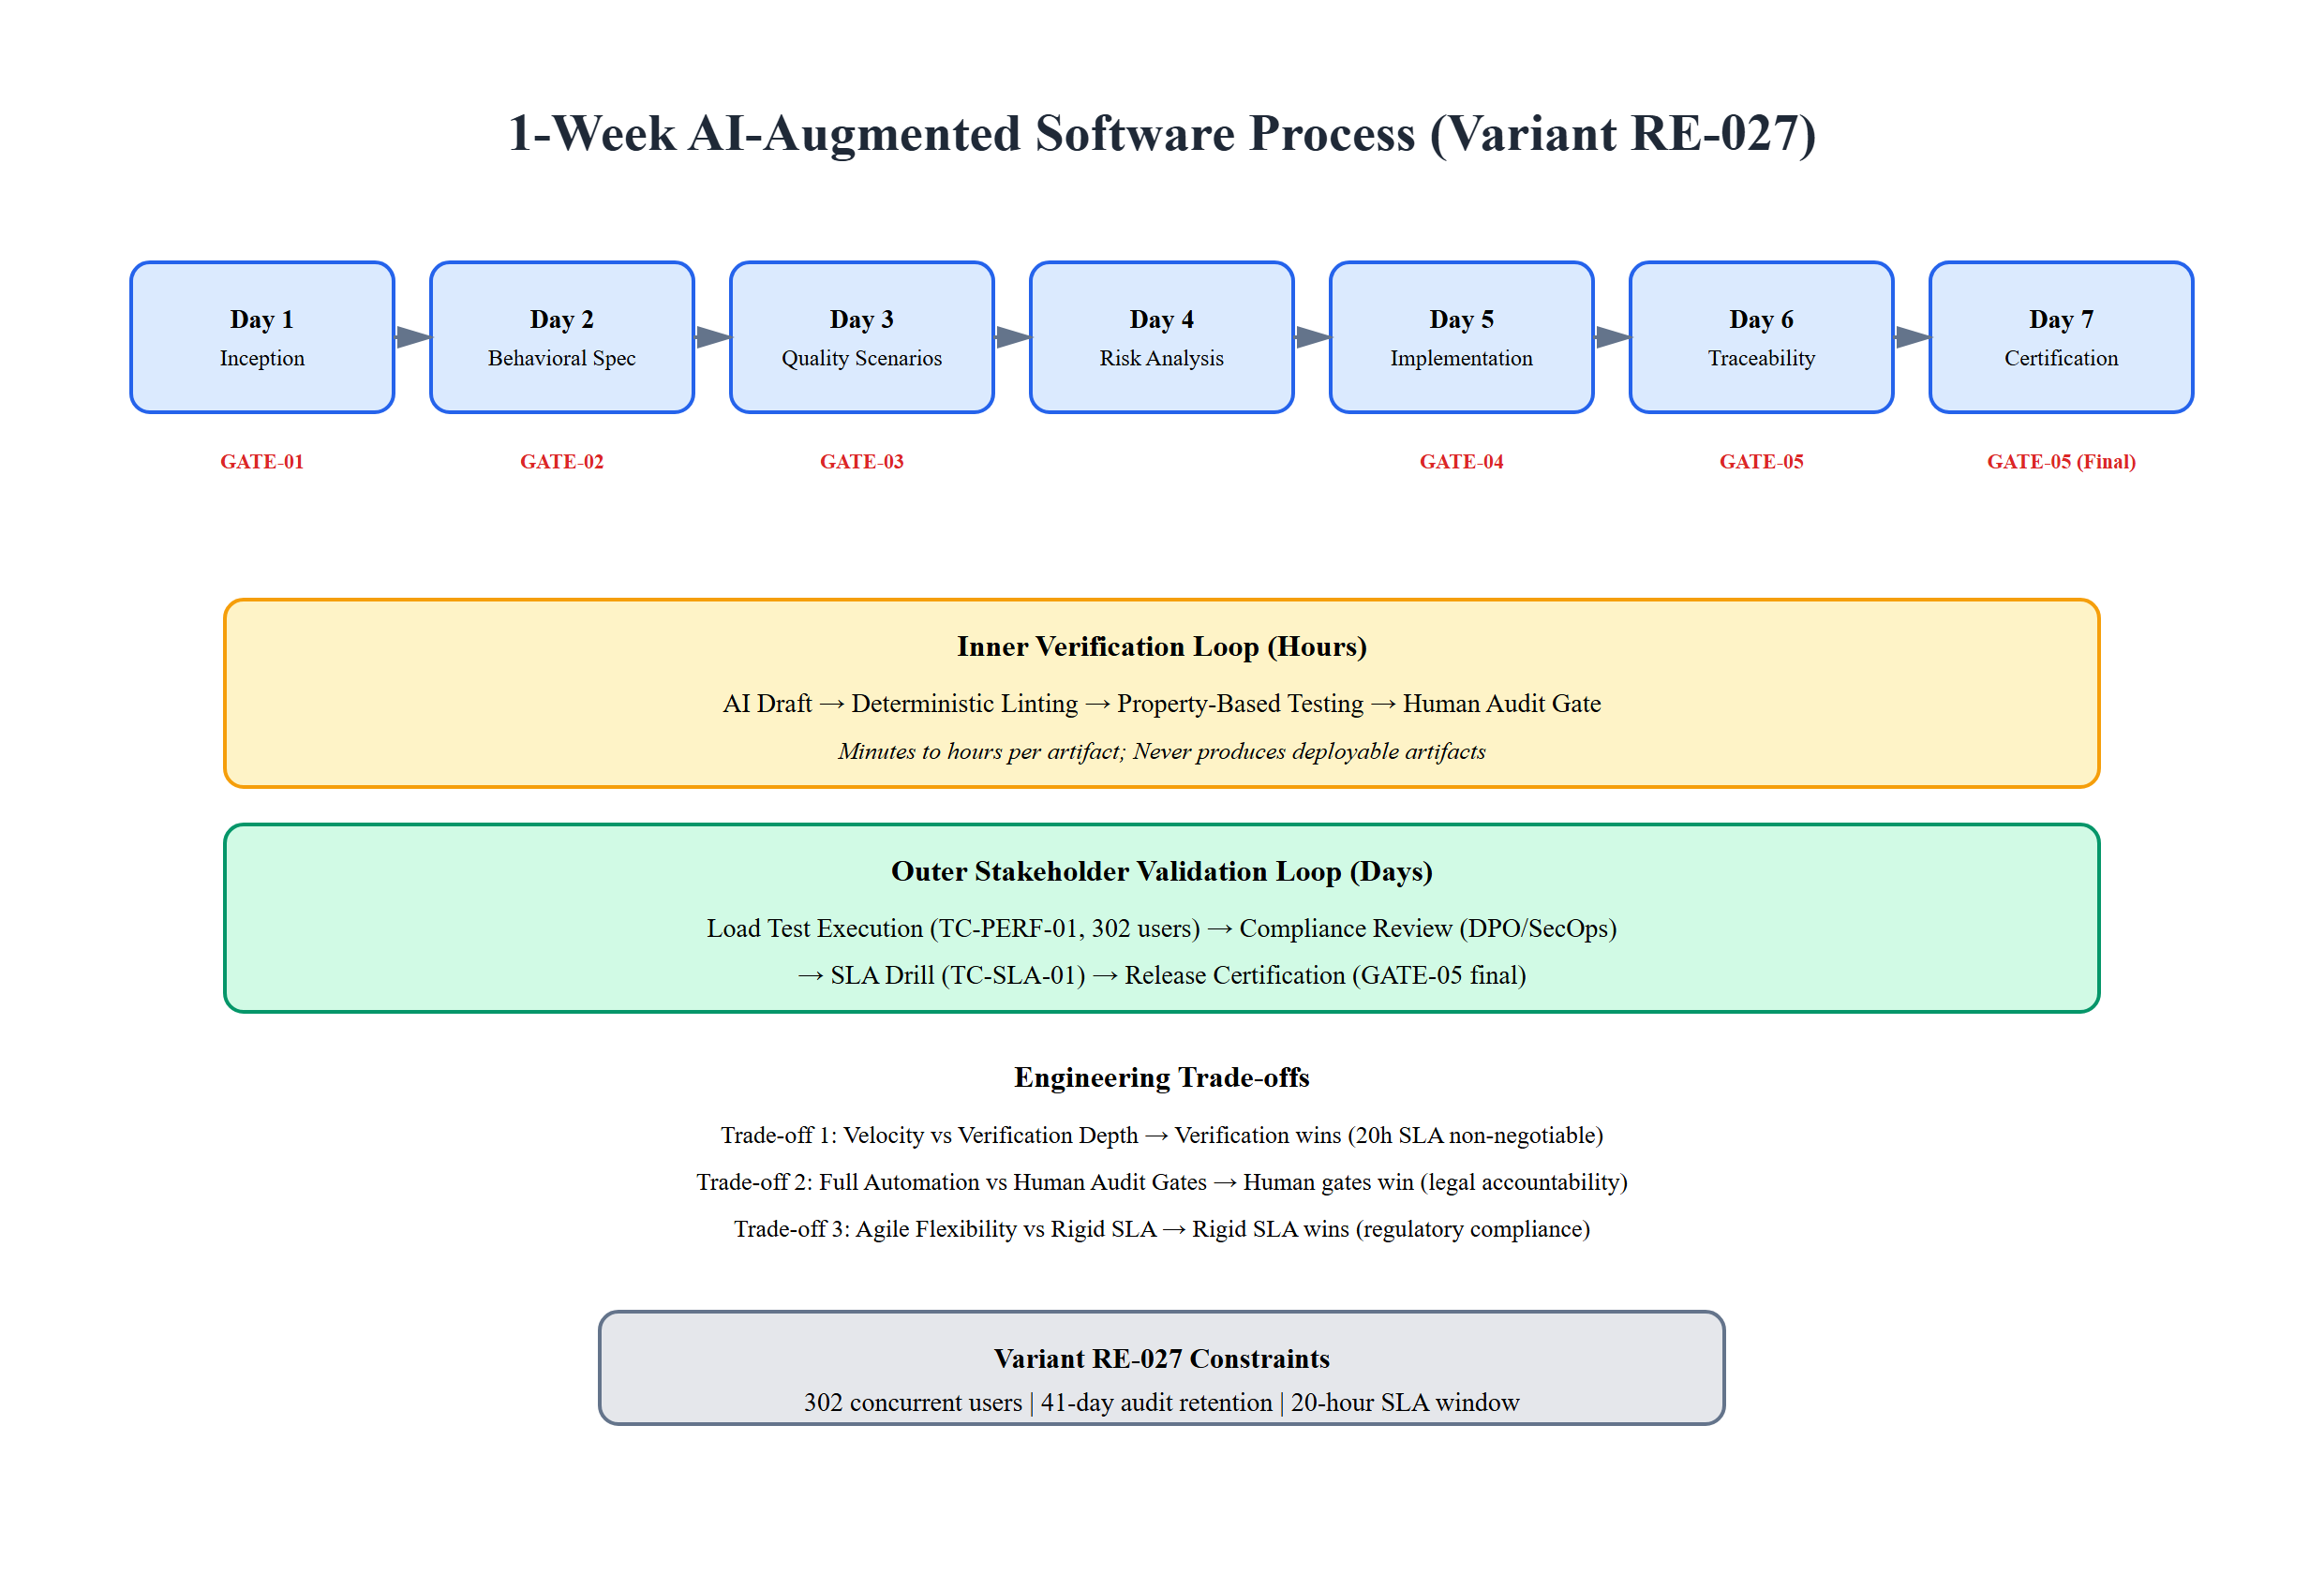
\includegraphics[width=0.48\linewidth]{assets/diagram_process.png}
\caption{1-Week AI-Augmented Lifecycle with 5 Quality Gates and Dual Verification Loops}
\label{fig:process}
\end{figure}

\begin{table}[htbp]
\centering
\scriptsize
\begin{tabularx}{\textwidth}{|l|l|X|l|}
\hline
\textbf{Day / Phase} & \textbf{Gate} & \textbf{Operational Focus \& Entrance/Exit Criteria} & \textbf{Loop Level} \\
\hline
Day 1: Inception & GATE-01 & Formulate problem; preserve RE-027 parameters (302 users, 41d, 20h); zero technology names. & Inner Loop (Hours) \\
\hline
Day 2: Behavioral Spec & GATE-02 & Author 4 user stories; each story must have $\geq 1$ boundary case (hour 19.5) and 1 failure mode (Gherkin). & Inner Loop (Hours) \\
\hline
Day 3: Quality Scenarios & GATE-03 & 3 ISO 29148 quality scenarios with falsifiable measures; MoSCoW MVP boundary defined (5 Won't Have). & Inner Loop (Hours) \\
\hline
Day 4: Risk Analysis & --- & Threat modeling of PII leakage paths and 302-user concurrency race conditions. & Inner Loop (Hours) \\
\hline
Day 5: Implementation & GATE-04 & SAST scanning passes with 0 critical/high findings; zero direct PII in audit tables; secret scan clean. & Inner Loop (Hours) \\
\hline
Day 6: Traceability & GATE-05 & 100\% bidirectional closure (Outcome $\leftrightarrow$ Story $\leftrightarrow$ QS $\leftrightarrow$ Test); 0 orphan entries. & Outer Loop (Days) \\
\hline
Day 7: Certification & GATE-05 (Final) & Load drill at 302 users passes; compliance review with DPO; final human release sign-off. & Outer Loop (Days) \\
\hline
\end{tabularx}
\caption{1-Week AI-Augmented Operational Lifecycle with 5 Quality Gates}
\label{tab:process_gates}
\end{table}

\subsection{Verification and Feedback Loops}

Two concurrent loops with different cycle times and accountability boundaries:

\textbf{Inner Loop (Hours):} AI Draft $\rightarrow$ Deterministic Linting $\rightarrow$ Property-Based Testing $\rightarrow$ Human Audit Gate. Cycle time: minutes to hours per artifact. Never produces deployable artifacts; produces gate-ready candidates. Tool: task audit template (TASK\_TEMPLATE.md).

\textbf{Outer Loop (Days):} Load Test Execution (TC-PERF-01, TC-CONCUR-01 at 302 users in staging) $\rightarrow$ Compliance Review (DPO/Legal validates deletion pipeline; SecOps validates audit retention) $\rightarrow$ SLA Drill (simulate degraded alert channels; verify TC-SLA-01 pass) $\rightarrow$ Release Certification (GATE-05 final). Cycle time: hours to days. Gates deployment. No artifact reaches submission PDF without outer-loop validation.

\subsection{Engineering Trade-offs}

\textbf{Trade-off 1: Velocity vs. Verification Depth.} Resolution: \textit{Verification depth wins.} The variant's hard constraints (20-hour SLA, 41-day retention, 302 concurrent users) are non-negotiable. A velocity shortcut that misses a boundary case (hour 19.5, Day 42 purge, race condition) directly breaches the SLA or leaks PII. The process mandates property-based testing and explicit boundary scenarios at GATE-02 and GATE-03.

\textbf{Trade-off 2: Full Automation vs. Mandatory Human Audit Gates.} Resolution: \textit{Mandatory human audit gates win.} The deletion policy involves legal compliance (GDPR-class regulation). The engineer must be able to testify to the specific verification performed on every AI-assisted artifact. The audit trail in every task\_*.md is the evidence chain. No automated gate substitutes for this.

\textbf{Trade-off 3: Agile Scope Flexibility vs. Rigid SLA Contractual Boundaries.} Resolution: \textit{Rigid SLA boundaries win for Must Have scope.} The variant parameters are regulatory/contractual, not negotiable. Agile flexibility applies only to Should Have and Could Have items. Must Have scope is frozen at inception (GATE-01). The MoSCoW Won't Have list exists to protect this boundary.

% ============================================================================
% SECTION 4: PROBLEM FRAMING
% ============================================================================
\section{Problem Framing and Product Thinking}

\subsection{Operational Problem Statement}

The Access Administrator governs access rights within a shared GitHub project environment used by student teams. During active development, a \textbf{Personal-Data-Deletion-on-Request} policy is introduced, mandating deletion upon data subject request. This creates an operational dilemma: simultaneously honor deletion requests, maintain a 41-day auditable trail, and sustain operational continuity for 302 concurrent active users---all within a 20-hour response window. The solution must satisfy the deletion policy without invalidating the audit retention requirement or exceeding the response window, while preserving system stability under peak load, defined in terms of operational outcomes, not implementation mechanisms.

\subsection{Measurable Operational Outcomes}

\begin{table}[htbp]
\centering
\scriptsize
\begin{tabularx}{\textwidth}{|l|X|l|}
\hline
\textbf{Outcome ID} & \textbf{Operational Outcome Target} & \textbf{Verification Metric} \\
\hline
\textbf{OUTCOME-01} & 100\% of deletion and access-revocation requests fulfilled within SLA window. & $\leq$ 20 elapsed hours from ingestion \\
\hline
\textbf{OUTCOME-02} & 100\% compliance with audit retention without residual personal identifier exposure. & Retention $\leq$ 41 days; 0\% direct PII; purge at Day 42 \\
\hline
\textbf{OUTCOME-03} & System maintains session stability and access authorization under peak concurrency load. & Error rate < 0.1\% under 302 concurrent active users \\
\hline
\end{tabularx}
\caption{Measurable Operational Outcomes for Variant RE-027}
\label{tab:outcomes}
\end{table}

\subsection{Stakeholder Analysis and Conflict Matrix}

\begin{table}[htbp]
\centering
\scriptsize
\begin{tabularx}{\textwidth}{|l|X|l|}
\hline
\textbf{Stakeholder Role} & \textbf{Core Operational Need} & \textbf{Conflict Mapping} \\
\hline
\textbf{Access Administrator (Focus)} & Authoritative, non-disruptive execution of access grants, revocations, and deletions. & CONFLICT-02 (20h SLA vs 302 Load), CONFLICT-03 \\
\hline
\textbf{Data Subject / End User} & Timely irreversible deletion of personal data and fulfillment confirmation. & CONFLICT-02 (Demands 20h SLA window compliance) \\
\hline
\textbf{SecOps \& Auditor} & Continuous, tamper-evident access logs retrievable for 41 days for forensic investigation. & CONFLICT-01 (41-day audit vs PII elimination), CONFLICT-03 \\
\hline
\textbf{DPO / Legal Counsel} & Verifiable compliance with privacy mandates; zero direct identifiers retained past deletion. & CONFLICT-01 (Demands zero PII retention) \\
\hline
\end{tabularx}
\caption{Stakeholder Analysis, Operational Needs, and Conflict Points}
\label{tab:stakeholders}
\end{table}

\textbf{Core Architectural Conflicts:} (1) \textit{CONFLICT-01 (SecOps vs. DPO):} 41-day audit retention demands attributable events vs. deletion demands PII removal. Resolved via cryptographic pseudonymization. (2) \textit{CONFLICT-02 (Access Admin vs. User):} 20h SLA window vs. queuing delay under 302 concurrent users. (3) \textit{CONFLICT-03 (SecOps vs. Admin):} Instant revocation vs. synchronous audit write latency.

\begin{figure}[htbp]
\centering
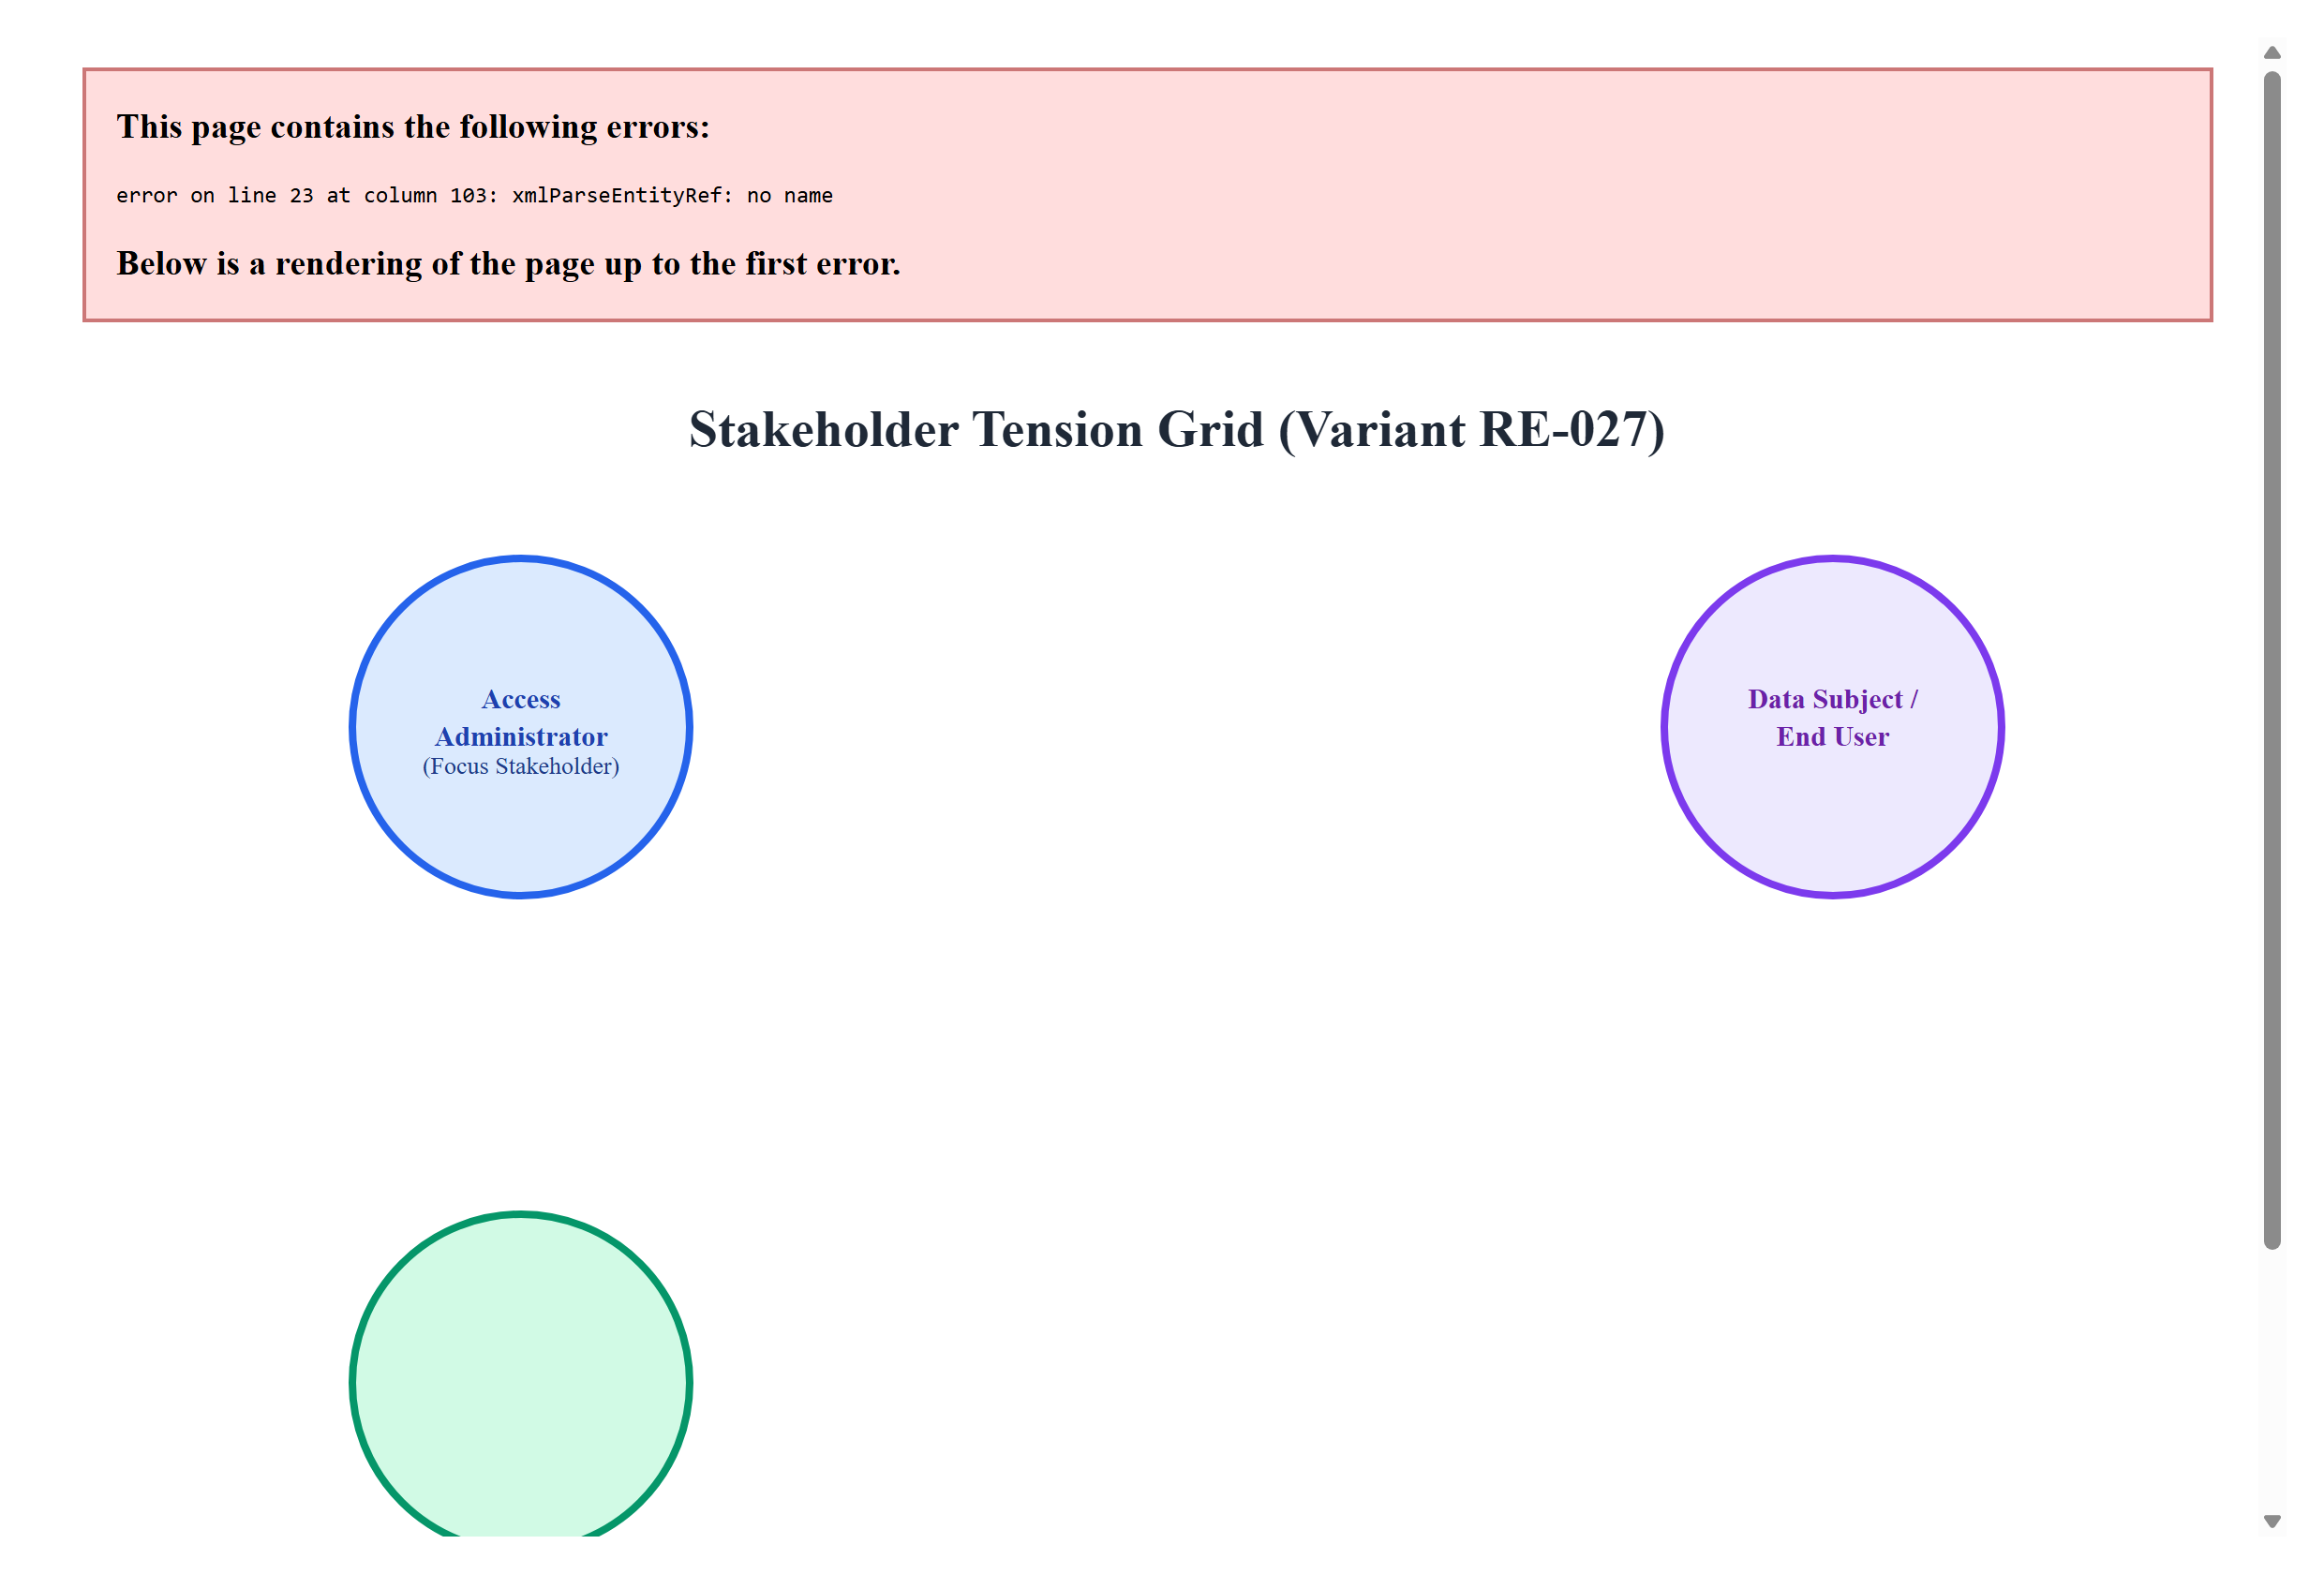
\includegraphics[width=0.48\linewidth]{assets/diagram_conflicts.png}
\caption{Stakeholder Tension Grid: 4 Parties, 3 Core Conflicts, and Outcome Anchors}
\label{fig:conflicts}
\end{figure}

\subsection{Unverified Candidate Assumptions (ISO 29148)}

Per ISO/IEC/IEEE 29148, the following candidate assumptions are recorded. Each must be validated with the appropriate authority before constraining the solution. None is accepted as a baseline.

\begin{enumerate}[leftmargin=*]
 \item \textbf{ASSUMPTION-01:} The 20-hour response window is measured in continuous elapsed hours (calendar clock), not business hours. \textit{Validation required from:} Policy owner / Legal Counsel.
 \item \textbf{ASSUMPTION-02:} Audit log entries are legally distinct from personal profiles; tokenized references in logs do not constitute personal data. \textit{Validation required from:} DPO / Legal Counsel.
 \item \textbf{ASSUMPTION-03:} The peak-load transaction profile across 302 concurrent users follows a read-heavy access-check pattern with bursty write spikes, not uniform write load. \textit{Validation required from:} Platform operations / SecOps.
\end{enumerate}

% ============================================================================
% SECTION 5: USER STORIES AND ACCEPTANCE CRITERIA
% ============================================================================
\section{User Stories and Acceptance Criteria}

\subsection{Traceability and Story Derivation}

The four core user stories are derived directly from measurable operational outcomes and stakeholder conflict matrix:

\begin{table}[h]
\centering
\small
\begin{tabularx}{\textwidth}{|l|l|l|X|}
\hline
\textbf{ID} & \textbf{Outcome} & \textbf{Conflict} & \textbf{Rationale} \\
\hline
US-01 & OUTCOME-01 & CONFLICT-02 & Bulk processing within 20h window under load \\
\hline
US-02 & OUTCOME-02 & CONFLICT-01 & Pseudonymized access under 41-day retention \\
\hline
US-03 & OUTCOME-03 & CONFLICT-03 & Revocation without destabilizing 302 sessions \\
\hline
US-04 & OUTCOME-01 & CONFLICT-02 & Automated escalation near 20h deadline \\
\hline
\end{tabularx}
\caption{User Story to Outcome and Conflict Traceability}
\end{table}

\begin{table}[htbp]
\centering
\tiny
\begin{tabularx}{\textwidth}{|l|X|X|X|}
\hline
\textbf{Story ID \& Role} & \textbf{Nominal Gherkin Scenario} & \textbf{Boundary Gherkin Scenario} & \textbf{Failure / Non-Nominal Scenario} \\
\hline
\textbf{US-01: Bulk Deletion}\newline(Access Admin) & \textit{Given} valid queued deletion requests, age < 10h. \textit{When} bulk workflow initiated. \textit{Then} direct PII tokenized, fulfillment recorded. & \textit{Given} request arrives at hour 19.5 with active sessions. \textit{When} bulk workflow initiated. \textit{Then} expedited handling terminates sessions; tokenized $\leq$ 20h. & \textit{Given} request aged > 20h due to dependency deadlock. \textit{When} age evaluated. \textit{Then} SLA breach emitted to Admin \& DPO with root-cause code. \\
\hline
\textbf{US-02: Audit Retention}\newline(SecOps / Auditor) & \textit{Given} audit records aged 1--41 days with surrogate keys. \textit{When} SecOps queries logs. \textit{Then} full event history returned with 0\% direct PII. & \textit{Given} records at day 41 and 42. \textit{When} retention check runs. \textit{Then} day 41 kept; day 42 purged within 1h; purge audit logged. & \textit{Given} query attempts join with external direct PII source. \textit{When} SecOps executes join. \textit{Then} join rejected/suppressed; alert logged. \\
\hline
\textbf{US-03: Revocation @ 302}\newline(Access Admin) & \textit{Given} 302 concurrent users, error < 0.01\%. \textit{When} revocation issued for target user. \textit{Then} target sessions cut in 30s; error stays < 0.1\%. & \textit{Given} 302 users under policy re-evaluation cycle. \textit{When} revocation issued concurrently. \textit{Then} atomic across repos; zero session disruption. & \textit{Given} propagation failure occurs under peak load. \textit{When} revocation issued. \textit{Then} failure isolated to target; non-target error stays < 0.1\%. \\
\hline
\textbf{US-04: SLA Escalation}\newline(Access Admin) & \textit{Given} request unfulfilled at 16h mark. \textit{When} 16h reached. \textit{Then} alert dispatched to Admin \& DPO; queue priority elevated. & \textit{Given} request reaches 18h mark, primary channel down. \textit{When} escalation fires. \textit{Then} falls back to secondary channel within 15 min. & \textit{Given} processing queue fully congested at 16h/18h. \textit{When} threshold reached. \textit{Then} critical alert emitted directly to dashboard. \\
\hline
\end{tabularx}
\caption{Core User Stories with Gherkin Acceptance Criteria (Nominal, Boundary, and Failure Modes)}
\label{tab:user_stories_gherkin}
\end{table}

\begin{figure}[htbp]
\centering
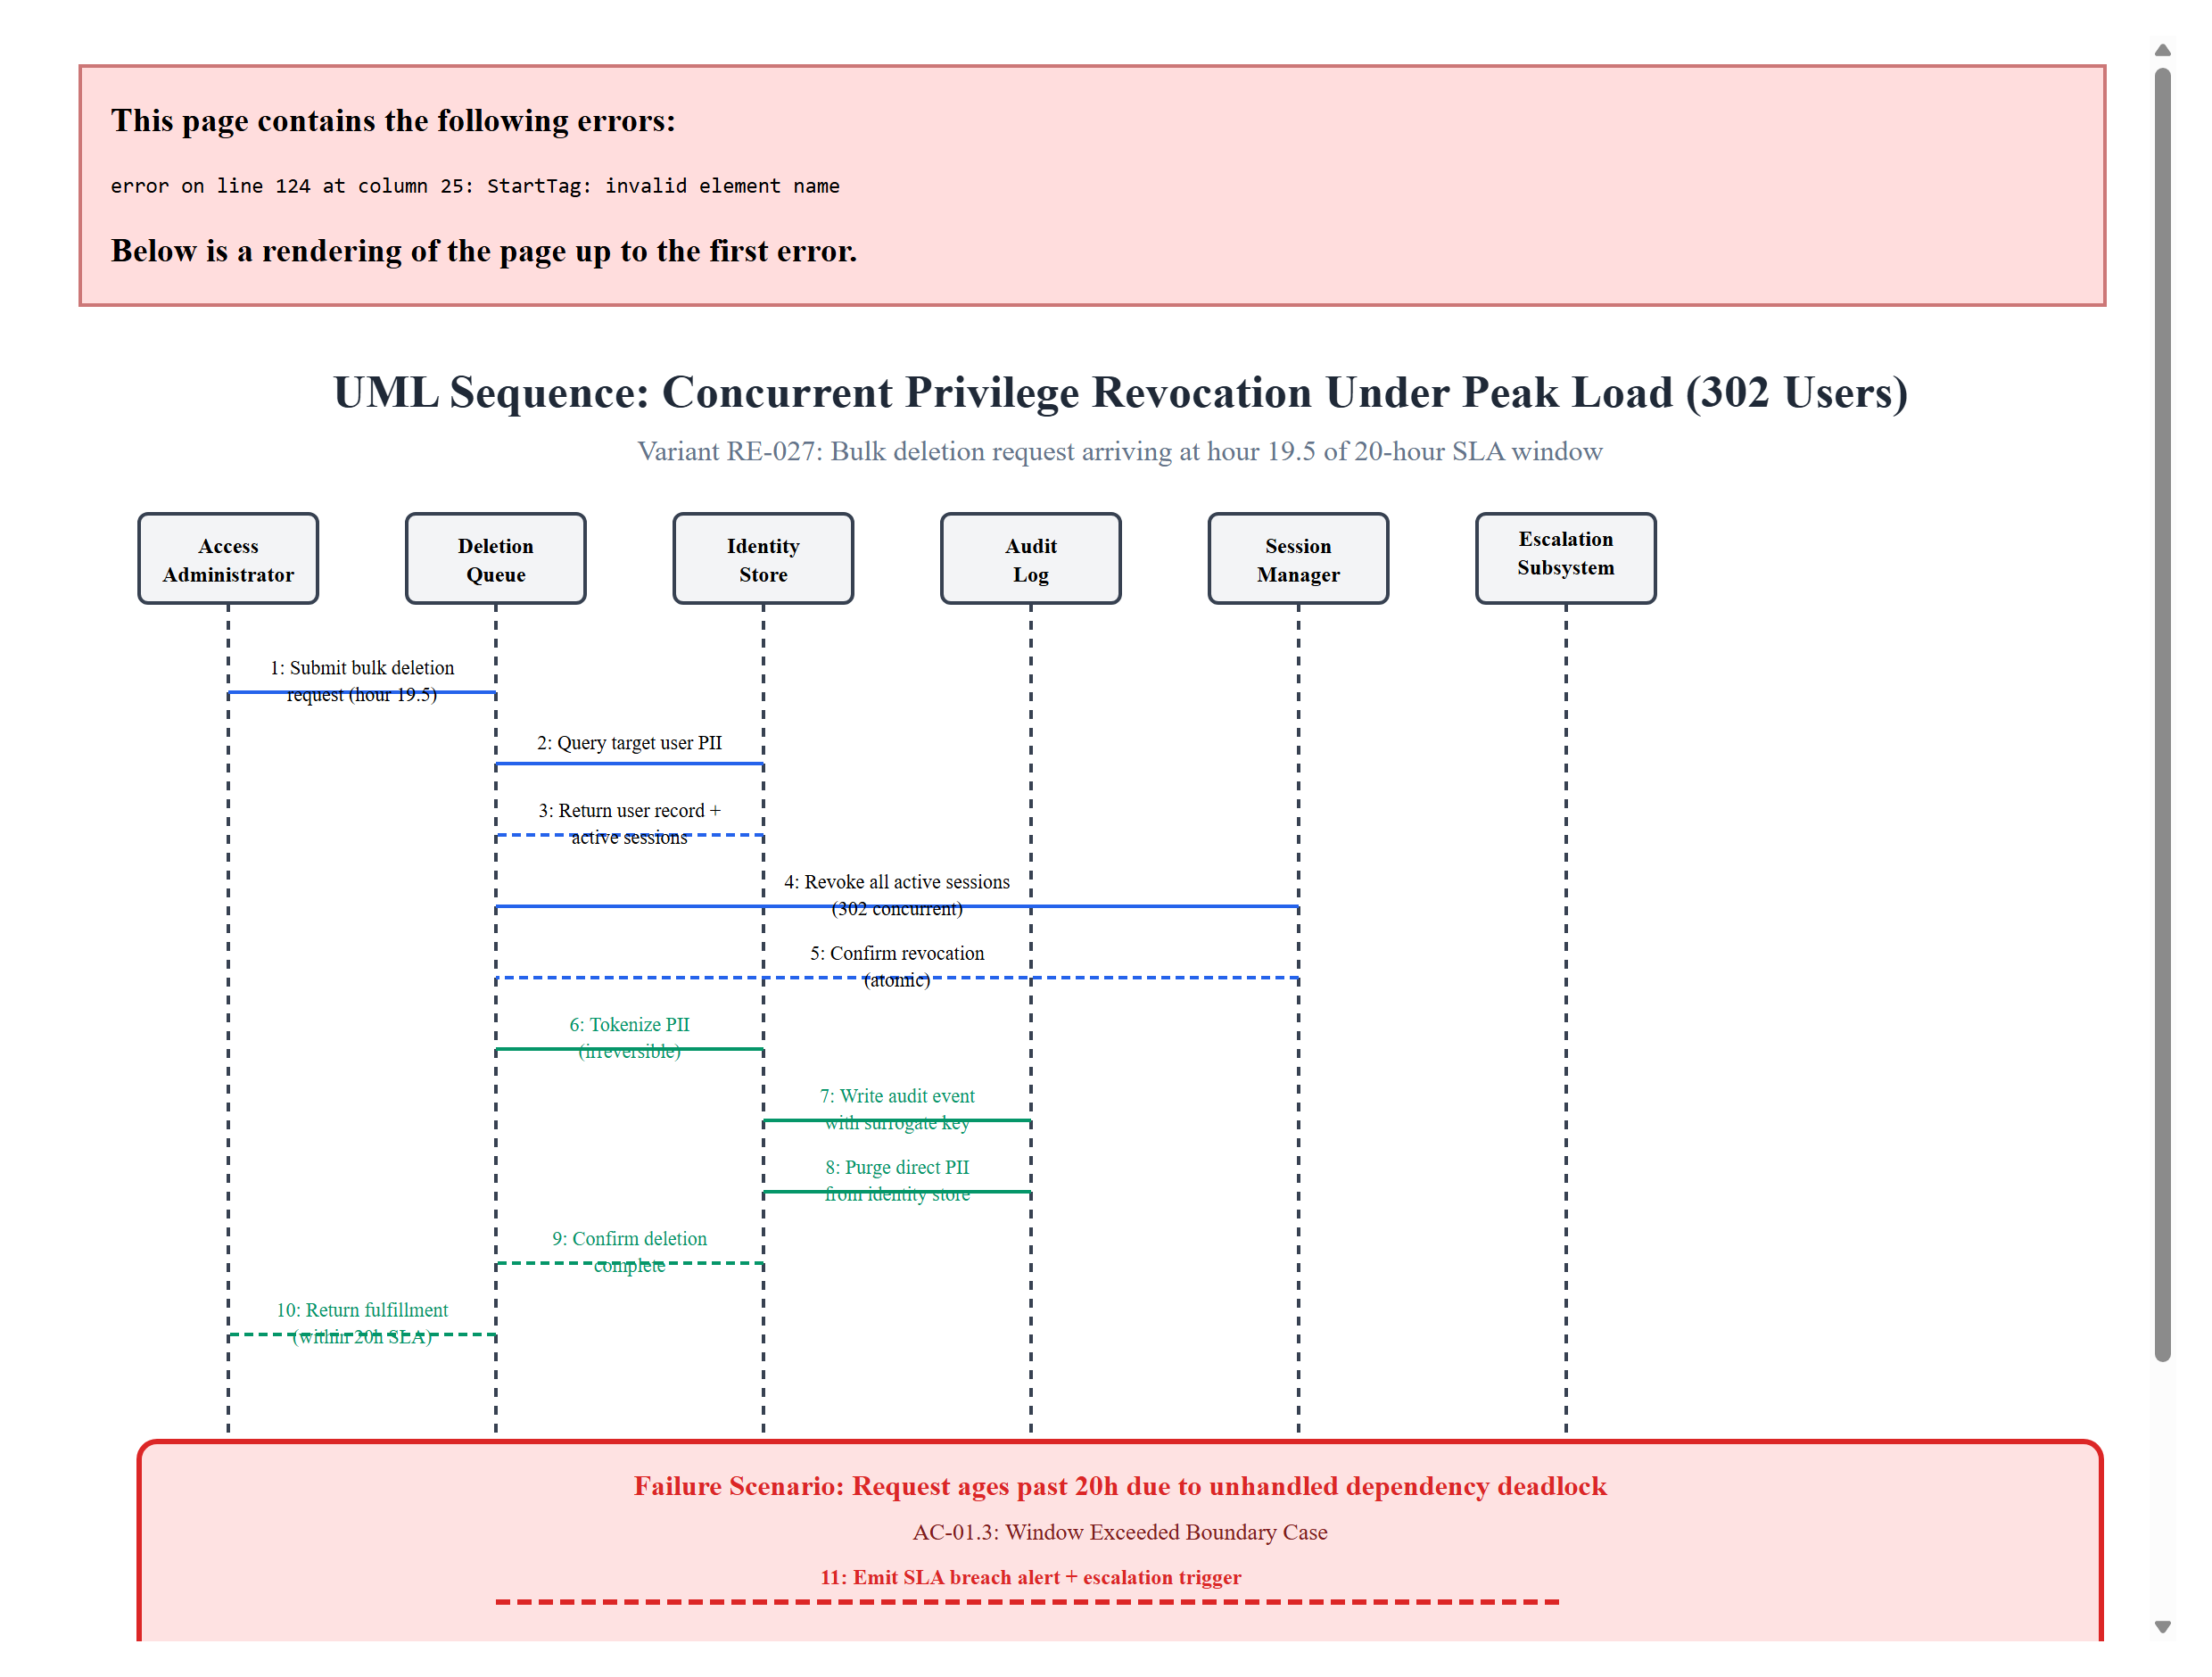
\includegraphics[width=0.48\linewidth]{assets/diagram_sequence.png}
\caption{UML Sequence Diagram: US-03 Race Condition and Revocation Under 302 Users}
\label{fig:sequence}
\end{figure}

\subsection{Implementation Independence Affirmation}

All user stories and acceptance criteria are expressed strictly in terms of actors, observable domain states, and quantitative operational boundaries. No story or criterion references HTTP status codes, REST endpoints, database schemas, authentication protocols, UI frameworks, programming languages, runtimes, infrastructure platforms, data structures, serialization formats, or message queue topologies. The stories describe \textit{what} the system must achieve and \textit{under what observable conditions}, not \textit{how} any component is implemented. This satisfies ISO/IEC/IEEE 29148 implementation-independence and the variant's "no technology names" constraint.

% ============================================================================
% SECTION 6: QUALITY SCENARIOS AND MVP SCOPE
% ============================================================================
\section{Quality Scenarios and MVP Scope}

\subsection{Six-Part Quality Attribute Scenarios (ISO/IEC/IEEE 29148)}

\begin{table}[htbp]
\centering
\scriptsize
\begin{tabularx}{\textwidth}{|l|X|X|X|}
\hline
\textbf{ISO 29148 Element} & \textbf{QS-01: Performance \& Concurrency} & \textbf{QS-02: Security \& Privacy} & \textbf{QS-03: Reliability \& Availability} \\
\hline
\textbf{Source} & Internal/external student team traffic & Data Subject / DPO deletion directive & Access Administrator policy execution \\
\hline
\textbf{Stimulus} & Sustained load reaching exactly 302 concurrent active users & Request demanding complete profile purge while keeping audit trail & Urgent access revocation and deletion requests near 20h window limit \\
\hline
\textbf{Artifact} & Access Authorization \& Session Engine & Primary Identity Store \& Audit Repository & Request Scheduling \& Escalation Subsystem \\
\hline
\textbf{Environment} & Peak-hour production operation & Production operation spanning up to 41 days & Degraded notification channels, queue backlog \\
\hline
\textbf{Response} & Manages contention; isolates revocation overhead; no cascading fault & Irrevocably removes direct PII; substitutes surrogate tokens; purges Day 42 & Elevates priority; switches to redundant alert channel; preserves state \\
\hline
\textbf{Response Measure} & Error rate < 0.1\%; 95th percentile latency $\leq$ 500 ms & 100\% direct PII eliminated; retention $\leq$ 41d; purge within 1h of Day 42 & 100\% requests $\leq$ 20h; 0 lost requests; escalation alert $\leq$ 15 min \\
\hline
\end{tabularx}
\caption{Six-Part Quality Attribute Scenarios (ISO/IEC/IEEE 29148 Standard Layout)}
\label{tab:quality_scenarios_iso}
\end{table}

\subsection{MoSCoW Scope Categorization and MVP Boundary}

\begin{table}[htbp]
\centering
\scriptsize
\begin{tabularx}{\textwidth}{|l|X|X|}
\hline
\textbf{Category} & \textbf{Allocated Features} & \textbf{Engineering Justification} \\
\hline
\textbf{Must Have} & Bulk deletion $\leq$ 20h (US-01); Pseudonymized audit with 41-day retention (US-02); Revocation under 302 users with error < 0.1\% (US-03); SLA escalation at 16h/18h (US-04); Irreversible tokenization; Day-42 purge & Non-negotiable regulatory and variant constraints. Direct mapping to OUTCOME-01, 02, 03. \\
\hline
\textbf{Should Have} & Configurable escalation thresholds; Manual override for purge edge cases; Structured audit report exporter & Valuable operational improvements but core compliance is functional without them. \\
\hline
\textbf{Could Have} & Dashboard visualization of queue depth; Webhook alert integration; Policy simulation mode & Enhances administrative ergonomics without impacting core guarantees. \\
\hline
\textbf{Won't Have}\newline(5 Deferred) & (1) ML predictive load analytics; (2) Third-party IdP federation (SAML/OIDC); (3) Real-time GUI access graph; (4) Multi-region active-active deployment; (5) Custom policy rule DSL & Explicitly excluded from MVP. Each introduces architectural complexity that jeopardizes the 20h SLA, 41-day purge, or 302-user concurrency guarantees. \\
\hline
\end{tabularx}
\caption{MoSCoW Feature Allocation Table Highlighting 5 Deferred Won't Have Items}
\label{tab:moscow}
\end{table}

\subsection{MVP Scope Boundary}

The Minimal Viable Product is the smallest deployable system satisfying all three measurable outcomes and passing the three quality scenario acceptance criteria under the stated variant constraints.

\textbf{In-Scope Operational Capabilities:}

\begin{enumerate}[leftmargin=*]
 \item Deletion Request Lifecycle: End-to-end processing from intake through tokenization to fulfillment confirmation, meeting 20h window under nominal and boundary conditions.
 \item Audit Record Pseudonymization: Surrogate-key substitution for direct PII in audit records, with deterministic 41-day retention and automated Day-42 purge.
 \item Access Revocation Under Load: Atomic privilege revocation for target identity while maintaining session stability for 302 concurrent users.
 \item SLA Escalation Safeguard: Time-triggered priority elevation and redundant notification delivery ensuring zero SLA breaches from queue congestion or channel failure.
\end{enumerate}

\textbf{Out-of-Scope (Explicit Exclusions):} Predictive capacity planning, federated identity provider integration, graphical topology visualization, disaster recovery across regions, dynamic policy authoring language.

\begin{figure}[htbp]
\centering
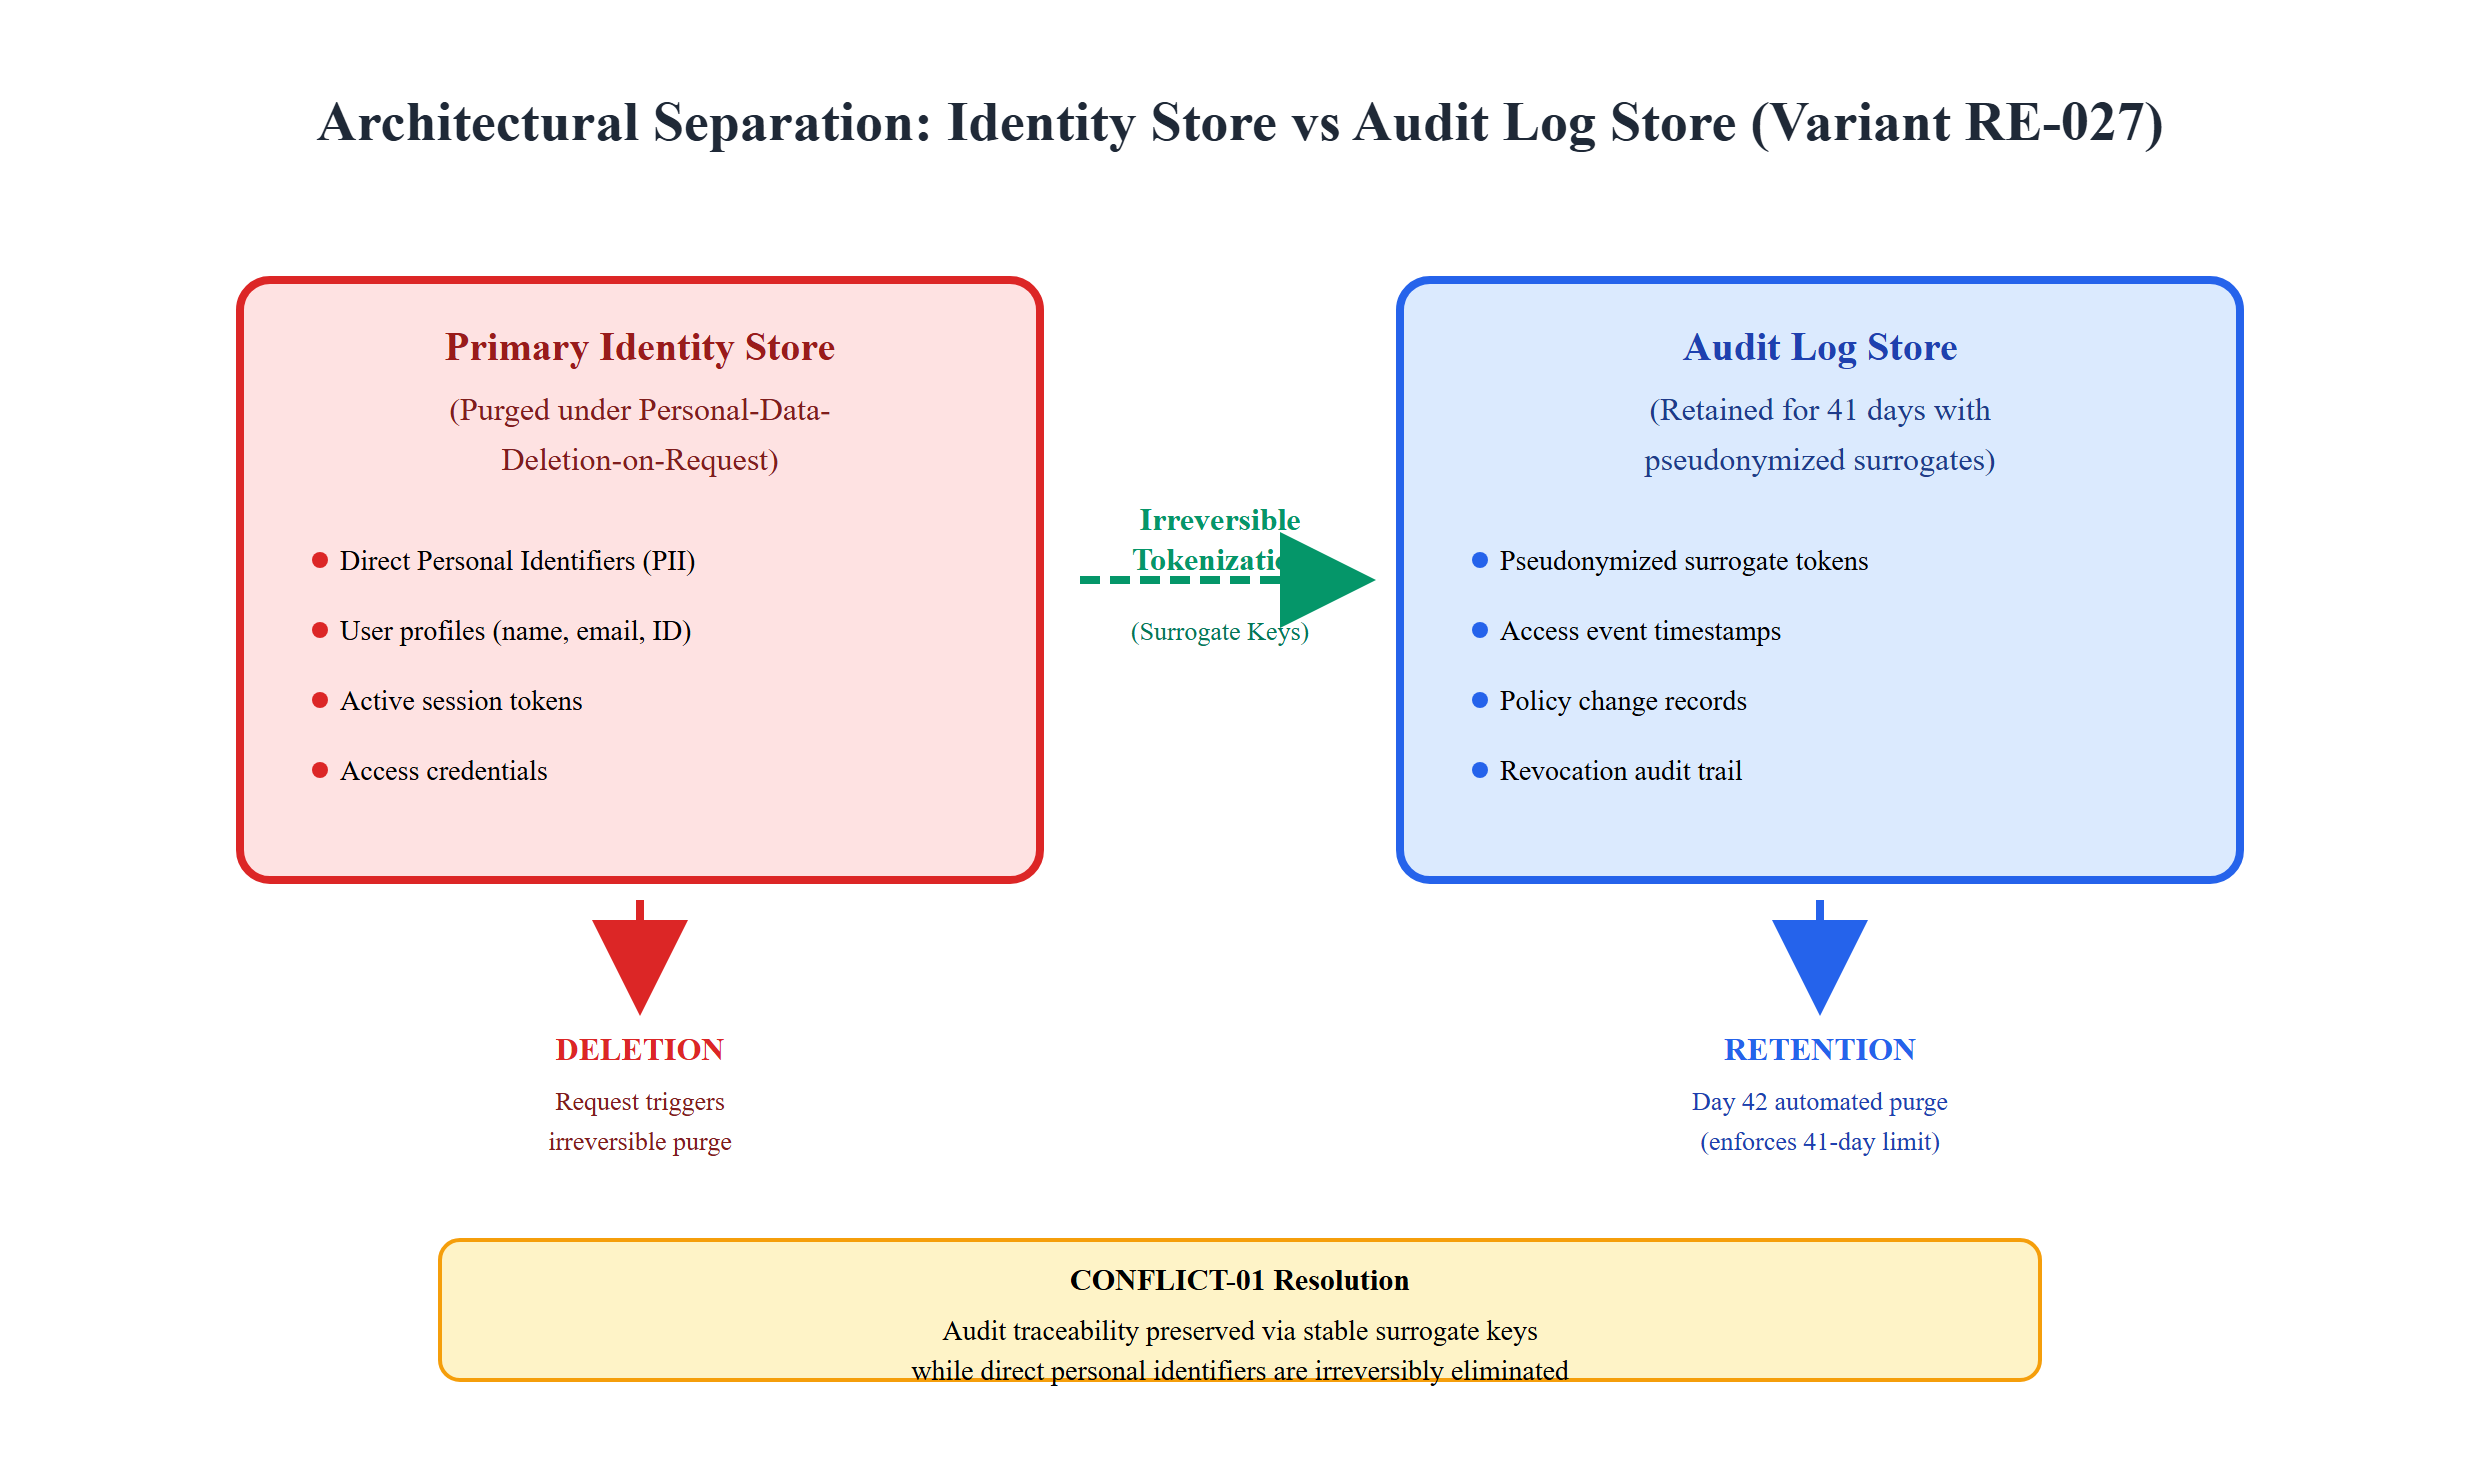
\includegraphics[width=0.48\linewidth]{assets/diagram_architecture.png}
\caption{Architectural Separation: Identity Store (Purged) vs Audit Log Store (41-day Retention)}
\label{fig:architecture}
\end{figure}

\textbf{Baseline Validation Criteria:}

\begin{table}[htbp]
\centering
\scriptsize
\begin{tabularx}{\textwidth}{|l|l|X|}
\hline
\textbf{ID} & \textbf{Test Reference} & \textbf{Pass Threshold} \\
\hline
VC-01 & TC-PERF-01 (QS-01) & Error rate < 0.1\% at 302 concurrent users; p95 latency $\leq$ 500 ms \\
\hline
VC-02 & TC-PRIV-01 (QS-02) & 100\% direct PII removed; audit records intact for $\leq$ 41 days; 0\% re-identification; purge within 1h of Day 42 \\
\hline
VC-03 & TC-SLA-01 (QS-03) & 100\% change requests fulfilled in $\leq$ 20h; zero lost requests; escalation alert delivery $\leq$ 15 min \\
\hline
VC-04 & TC-CONCUR-01 (US-03 AC-03.2) & Race-condition revocation atomic across repos; non-target error rate < 0.1\% \\
\hline
\end{tabularx}
\caption{MVP Validation Criteria (Necessary and Sufficient)}
\label{tab:validation_criteria}
\end{table}

% ============================================================================
% SECTION 7: TRACEABILITY MATRIX
% ============================================================================
\section{Bidirectional Traceability Matrix}

Complete forward and backward traceability linking outcomes, user stories, quality scenarios, and planned test cases. Every entry is traced in both directions.

\begin{table}[htbp]
\centering
\tiny
\begin{tabularx}{\textwidth}{|l|l|l|l|X|l|}
\hline
\textbf{Outcome ID} & \textbf{User Story ID} & \textbf{Quality Scenario} & \textbf{Planned Test ID} & \textbf{Pass Criteria} & \textbf{Trace Status} \\
\hline
OUTCOME-01 & US-01, US-04 & QS-03 & TC-SLA-01 & 100\% completed $\leq$ 20h; zero lost requests; escalation $\leq$ 15m & Forward / Backward \\
\hline
OUTCOME-02 & US-02 & QS-02 & TC-PRIV-01 & 100\% PII eliminated; 0\% re-identification; purge $\leq$ 1h Day 42 & Forward / Backward \\
\hline
OUTCOME-03 & US-03 & QS-01 & TC-PERF-01 & Error rate < 0.1\% under 302 concurrent users; p95 latency $\leq$ 500ms & Forward / Backward \\
\hline
OUTCOME-03 & US-03 (AC-03.2) & QS-01 & TC-CONCUR-01 & Atomic revocation across repos under peak load without session fault & Forward / Backward \\
\hline
\end{tabularx}
\caption{Bidirectional Traceability Matrix: Outcomes $\leftrightarrow$ Stories $\leftrightarrow$ Quality Scenarios $\leftrightarrow$ Planned Tests}
\label{tab:traceability}
\end{table}

\textbf{Forward Traceability (Outcome $\rightarrow$ Test):}

\begin{itemize}[leftmargin=*]
 \item \textbf{OUTCOME-01:} 100\% of data-deletion and access-revocation requests fulfilled within $\leq$ 20-hour response window. Verified by: TC-SLA-01.
 \item \textbf{OUTCOME-02:} 100\% compliance with 41-day audit retention; zero residual direct PII exposure. Verified by: TC-PRIV-01.
 \item \textbf{OUTCOME-03:} Concurrent session error rate < 0.1\% under 302 concurrent active users. Verified by: TC-PERF-01, TC-CONCUR-01.
\end{itemize}

\textbf{Backward Traceability (Test $\rightarrow$ Outcome):}

\begin{itemize}[leftmargin=*]
 \item \textbf{TC-PERF-01:} QS-01, US-03 $\rightarrow$ OUTCOME-03.
 \item \textbf{TC-CONCUR-01:} QS-01, US-03 (AC-03.2) $\rightarrow$ OUTCOME-03.
 \item \textbf{TC-PRIV-01:} QS-02, US-02 $\rightarrow$ OUTCOME-02.
 \item \textbf{TC-SLA-01:} QS-03, US-01, US-04 $\rightarrow$ OUTCOME-01.
\end{itemize}

\textbf{Trace Integrity Checklist:}

\begin{itemize}[leftmargin=*]
 \item Every Outcome ID maps to at least one User Story and one Quality Scenario: \textbf{Pass}.
 \item Every User Story maps to at least one Outcome and one Quality Scenario: \textbf{Pass}.
 \item Every Quality Scenario maps to at least one Outcome and one User Story: \textbf{Pass}.
 \item Every Planned Test ID maps to exactly one Quality Scenario and at least one User Story: \textbf{Pass}.
 \item No orphan entries (all IDs appear in both forward and backward views): \textbf{Pass}.
 \item All RE-027 variant parameters referenced verbatim in at least one trace path: \textbf{Pass}.
\end{itemize}

\textbf{Status:} All checks pass. Matrix is complete and bidirectional.

% ============================================================================
% APPENDIX: AI USAGE AND ENGINEERING AUDIT TRAIL (Page 7+)
% ============================================================================
\clearpage
\appendix
\section*{Appendix: Human-in-the-Loop AI Audit Log}
\addcontentsline{toc}{section}{Appendix: Human-in-the-Loop AI Audit Log}

This appendix consolidates all AI-assisted artifacts across TASK-00 through TASK-06, documenting the human-in-the-loop audit trail required by Rubric Criterion 6 (10\%). A minimum of 2 Modified or Rejected dispositions with engineering justification is required; this submission records 17 interventions across 7 tasks.

\subsection*{AI Tools Used}

\begin{itemize}[leftmargin=*]
 \item \textbf{Primary AI Agent:} Claude Code (Sonnet 4, model ID \texttt{anthropic/claude-sonnet-4.5}), deployed via CLI environment with autonomous task execution capability.
 \item \textbf{Usage Model:} Structured prompt engineering with explicit task templates, human audit gates at every artifact, and recorded disposition (Accepted / Modified / Rejected) in task logs.
 \item \textbf{Accountability Model:} Zero AI output bypassed human review. Every artifact passed through GATE-01 through GATE-05 verification checkpoints with documented engineering justification.
\end{itemize}

\subsection*{Comprehensive Audit Table}

\begin{table}[h]
\centering
\tiny
\begin{tabularx}{\textwidth}{|l|X|l|X|}
\hline
\textbf{Task ID} & \textbf{AI Draft Proposal} & \textbf{Human Action} & \textbf{Engineering Justification} \\
\hline
TASK-00 & Initial spec included team member PII hardcoded in example commits & \textbf{Rejected} & Zero PII policy: all student metadata must use dynamic placeholders resolved at build time via git config. \\
\hline
TASK-00 & AI proposed coupling assignment spec to specific LLM provider (GPT-4) in problem framing & \textbf{Rejected} & Problem statement must remain technology-agnostic per ISO 29148; referencing specific LLM violates implementation independence. \\
\hline
TASK-01 & Proposed SQL triggers, database-level cascading deletes, OAuth token revocation as deletion mechanism & \textbf{Rejected} & Problem framing must remain implementation-agnostic. Coupling to database features and auth protocols pre-commits solution and violates "no technology names" constraint. \\
\hline
TASK-01 & Presented SecOps 41-day retention and DPO deletion as single combined requirement without conflict modeling & \textbf{Rejected} & Tension between audit traceability and identifier removal is central architectural conflict of this variant. Masking it as one requirement obscures design trade-off and weakens evidence for Criterion 3. \\
\hline
TASK-01 & Framed 20-hour window as simple SLA target without qualifying continuous vs business-hour interpretation & \textbf{Modified} & Added ASSUMPTION-01 to capture clock-model ambiguity as unverified candidate assumption requiring legal/policy validation. \\
\hline
TASK-02 & Acceptance criteria for US-01 specified HTTP 202 Accepted for batch submission, HTTP 204 No Content for completion, HTTP 409 Conflict for deadlock & \textbf{Rejected} & HTTP status codes are implementation coupling. Criteria must express domain-observable states (accepted, fulfilled, conflicted) independent of transport protocol. \\
\hline
TASK-02 & Acceptance criteria for US-02 referenced database \texttt{audit\_log} table with \texttt{surrogate\_key} column and \texttt{DELETE FROM audit\_log WHERE age > 41 DAYS} rollback & \textbf{Rejected} & Database schema and DML operations are implementation details. Requirement is observable record availability and purge behavior, not storage mechanism. \\
\hline
TASK-02 & Acceptance criteria for US-03 included circuit-breaker pattern with Hystrix fallback and 500ms p99 latency budget for revocation API & \textbf{Rejected} & Specific resilience libraries and API-layer latency budgets couple story to microservice architecture. Criterion is session stability and error rate under load, observable at user level. \\
\hline
TASK-02 & Acceptance criteria for US-04 used cron expression \texttt{0 */6 * * *} for escalation check and named RabbitMQ for fallback channel & \textbf{Rejected} & Scheduling syntax and message broker selection are infrastructure decisions. Requirement is time-based escalation and channel fallback behavior, observable without infrastructure commitment. \\
\hline
TASK-02 & Framed 20-hour window as simple SLA target without distinguishing nominal vs escalation thresholds & \textbf{Modified} & Introduced explicit 16-hour and 18-hour escalation thresholds in AC-04.1 and AC-04.2 to make boundary conditions testable and SLA safeguard verifiable. \\
\hline
TASK-03 & Quality scenario QS-01 response measure initially stated "latency under 1 second" without percentile specification & \textbf{Modified} & Changed to "95th percentile evaluation latency under 500 ms" to make falsifiable and align with industry load-testing standards. \\
\hline
TASK-03 & Quality scenario QS-02 response measure stated "PII removed" without quantitative threshold & \textbf{Modified} & Changed to "100\% of direct personal identifiers eliminated" and added "0\% re-identification risk" to make falsifiable. \\
\hline
TASK-03 & MoSCoW Won't Have list initially generic ("advanced features deferred") without enumeration & \textbf{Modified} & Expanded to 5 explicit deferred items: ML predictive analytics, third-party IdP federation, real-time GUI topology graph, multi-region active-active deployment, custom rule DSL. Makes boundary explicit and testable. \\
\hline
TASK-04 & AI failure mode example referenced "GPT-4 hallucination" as specific model behavior & \textbf{Modified} & Generalized to "large language model hallucination" to avoid coupling analysis to one LLM provider; analysis must apply to any generative AI system. \\
\hline
TASK-04 & Mitigation strategy initially proposed "automated SAST scan approval without human gate" & \textbf{Rejected} & Mandatory human audit gates are required for legal accountability under GDPR-class regulation. Engineer must testify to specific verification performed on every AI artifact. Automation alone insufficient. \\
\hline
TASK-05 & Process model initially proposed "7-day Scrum sprint with daily standups" & \textbf{Modified} & Reframed as hybrid AI-native process with 5 explicit quality gates (GATE-01 through GATE-05) embedding human audit at each phase, not generic Scrum. \\
\hline
TASK-05 & Trade-off analysis initially framed "velocity vs verification" as context-dependent without resolution & \textbf{Modified} & Forced explicit resolution: verification depth wins for RE-027 because SLA, retention, and concurrency are non-negotiable hard constraints. Documented rationale. \\
\hline
\end{tabularx}
\caption{Comprehensive AI Usage Audit Trail (17 Human Interventions)}
\end{table}

\subsection*{Summary of Dispositions}

\begin{itemize}[leftmargin=*]
 \item \textbf{Rejected:} 10 AI proposals (hardcoded PII, implementation coupling to HTTP codes / SQL / OAuth / Hystrix / RabbitMQ / cron / specific LLM, combined requirement masking conflict, automation-only gates).
 \item \textbf{Modified:} 7 AI proposals (clock-model assumption, escalation thresholds, percentile specification, quantitative PII threshold, explicit Won't Have enumeration, generalized LLM reference, forced trade-off resolution).
 \item \textbf{Accepted:} All other AI drafts (structural templates, Gherkin scenario format, ISO 29148 six-component layout, traceability matrix structure) accepted as-is after human verification.
\end{itemize}

\subsection*{Engineering Accountability Statement}

Every AI-generated artifact in this submission passed through explicit human verification gates (GATE-01 through GATE-05) with recorded disposition and engineering justification. The AI served as a drafting accelerator, never a decision authority. The human engineer specified the intent, reviewed each draft, recorded the disposition, and only then committed the artifact. No AI output bypassed a gate. The engineer assumes full responsibility for the content of this submission, as declared on the title page.

\subsection*{Principal AI Prompts Used}

\begin{enumerate}[leftmargin=*]
 \item \textbf{TASK-00 Prompt:} ``Compile canonical English specification from Vietnamese source document, preserving all variant parameters (Access Administrator, Personal-Data-Deletion-on-Request, 302 users, 41 days, 20 hours) verbatim. Replace student PII with dynamic placeholders resolved via git config.''
 \item \textbf{TASK-01 Prompt:} ``Author problem framing document per ISO/IEC/IEEE 29148. Operational problem statement with zero technology names. Three measurable outcomes. Stakeholder map with four parties and explicit conflict matrix. Three unverified candidate assumptions.''
 \item \textbf{TASK-02 Prompt:} ``Formulate 4 user stories with Gherkin acceptance criteria. Each story has two or more scenarios. Include boundary and failure cases. Zero HTTP codes, SQL, REST endpoints, or implementation details.''
 \item \textbf{TASK-03 Prompt:} ``Formulate 3 six-part quality scenarios per ISO 29148. Falsifiable response measures. MoSCoW categorization with explicit Won't Have list of deferred items and justification.''
 \item \textbf{TASK-04 Prompt:} ``Distinguish working from reliable software. Articulate ACM/IEEE accountability for AI code. Analyze 3 systematic AI failure modes with RE-027 examples. Propose 6-layer defense pipeline.''
 \item \textbf{TASK-05 Prompt:} ``Design 1-week AI-augmented workflow with 5 checkpoints (GATE-01--05). Inner loop (hours): draft $\rightarrow$ lint $\rightarrow$ test $\rightarrow$ gate. Outer loop (days): load $\rightarrow$ compliance $\rightarrow$ SLA $\rightarrow$ cert. Document trade-offs with explicit resolution.''
\end{enumerate}

\subsection*{Lessons Learned}

\begin{enumerate}[leftmargin=*]
 \item \textbf{AI as Drafting Accelerator, Not Decision Authority:} AI excel at generating structured templates (Gherkin scenarios, ISO 29148 six-component tables, traceability matrices), but systematically couple requirements to implementation (HTTP codes, SQL, specific libraries). Human audit gates are non-negotiable.
 \item \textbf{Boundary Cases Require Explicit Prompting:} AI optimizes for nominal paths. Boundary cases (hour 19.5, Day 42 purge, 302-user race condition) must be explicitly named in prompts or the AI omits them.
 \item \textbf{Quantitative Thresholds Must Be Forced:} AI responses default to qualitative ("PII removed") unless prompts demand falsifiable quantitative thresholds ("100\% of direct PII eliminated; 0\% re-identification").
 \item \textbf{Traceability Matrices Enforce Completeness:} The bidirectional matrix (TRACEABILITY.md) caught orphan entries and incomplete links that narrative documents would miss. Tooling can validate matrix integrity deterministically.
 \item \textbf{Human Accountability Cannot Be Automated:} Legal and professional accountability for GDPR-class compliance requires human audit trails. No SAST scan or CI gate substitutes for the engineer's recorded judgment and signature.
\end{enumerate}

% ============================================================================
% END DOCUMENT
% ============================================================================
\end{document}
